%**************************************%
%* Generated from MathBook XML source *%
%*    on 2016-08-20T09:15:12-04:00    *%
%*                                    *%
%*   http://mathbook.pugetsound.edu   *%
%*                                    *%
%**************************************%
\documentclass[10pt,]{article}
%% Load geometry package to allow page margin adjustments
\usepackage{geometry}
\geometry{letterpaper,total={5.0in,9.0in}}
%% Custom Preamble Entries, early (use latex.preamble.early)
%% Inline math delimiters, \(, \), need to be robust
%% 2016-01-31:  latexrelease.sty  supersedes  fixltx2e.sty
%% If  latexrelease.sty  exists, bugfix is in kernel
%% If not, bugfix is in  fixltx2e.sty
%% See:  https://tug.org/TUGboat/tb36-3/tb114ltnews22.pdf
%% and read "Fewer fragile commands" in distribution's  latexchanges.pdf
\IfFileExists{latexrelease.sty}{}{\usepackage{fixltx2e}}
%% Page Layout Adjustments (latex.geometry)
%% This LaTeX file may be compiled with pdflatex, xelatex, or lualatex
%% The following provides engine-specific capabilities
%% Generally, xelatex and lualatex will do better languages other than US English
%% You can pick from the conditional if you will only ever use one engine
\usepackage{ifthen}
\usepackage{ifxetex,ifluatex}
\ifthenelse{\boolean{xetex} \or \boolean{luatex}}{%
%% begin: xelatex and lualatex-specific configuration
%% fontspec package will make Latin Modern (lmodern) the default font
\ifxetex\usepackage{xltxtra}\fi
\usepackage{fontspec}
%% realscripts is the only part of xltxtra relevant to lualatex 
\ifluatex\usepackage{realscripts}\fi
%% 
%% Extensive support for other languages
\usepackage{polyglossia}
\setdefaultlanguage{english}
%% Magyar (Hungarian)
\setotherlanguage{magyar}
%% Spanish
\setotherlanguage{spanish}
%% Vietnamese
\setotherlanguage{vietnamese}
%% end: xelatex and lualatex-specific configuration
}{%
%% begin: pdflatex-specific configuration
%% translate common Unicode to their LaTeX equivalents
%% Also, fontenc with T1 makes CM-Super the default font
%% (\input{ix-utf8enc.dfu} from the "inputenx" package is possible addition (broken?)
\usepackage[T1]{fontenc}
\usepackage[utf8]{inputenc}
%% end: pdflatex-specific configuration
}
%% Monospace font: Inconsolata (zi4)
%% Sponsored by TUG: http://levien.com/type/myfonts/inconsolata.html
%% See package documentation for excellent instructions
%% One caveat, seem to need full file name to locate OTF files
%% Loads the "upquote" package as needed, so we don't have to
%% Upright quotes might come from the  textcomp  package, which we also use
%% We employ the shapely \ell to match Google Font version
%% pdflatex: "varqu" option produces best upright quotes
%% xelatex,lualatex: add StylisticSet 1 for shapely \ell
%% xelatex,lualatex: add StylisticSet 2 for plain zero
%% xelatex,lualatex: we add StylisticSet 3 for upright quotes
%% 
\ifthenelse{\boolean{xetex} \or \boolean{luatex}}{%
%% begin: xelatex and lualatex-specific monospace font
\usepackage{zi4}
\setmonofont[BoldFont=Inconsolatazi4-Bold.otf,StylisticSet={1,3}]{Inconsolatazi4-Regular.otf}
%% end: xelatex and lualatex-specific monospace font
}{%
%% begin: pdflatex-specific monospace font
\usepackage[varqu]{zi4}
%% end: pdflatex-specific monospace font
}
%% Symbols, align environment, bracket-matrix
\usepackage{amsmath}
\usepackage{amssymb}
%% allow more columns to a matrix
%% can make this even bigger by overriding with  latex.preamble.late  processing option
\setcounter{MaxMatrixCols}{30}
%%
%% Color support, xcolor package
%% Always loaded.  Used for:
%% mdframed boxes, add/delete text, author tools
\PassOptionsToPackage{usenames,dvipsnames,svgnames,table}{xcolor}
\usepackage{xcolor}
%%
%% Semantic Macros
%% To preserve meaning in a LaTeX file
%% Only defined here if required in this document
%% Used for inline definitions of terms
\newcommand{\terminology}[1]{\textbf{#1}}
%% Subdivision Numbering, Chapters, Sections, Subsections, etc
%% Subdivision numbers may be turned off at some level ("depth")
%% A section *always* has depth 1, contrary to us counting from the document root
%% The latex default is 3.  If a larger number is present here, then
%% removing this command may make some cross-references ambiguous
%% The precursor variable $numbering-maxlevel is checked for consistency in the common XSL file
\setcounter{secnumdepth}{3}
%% Environments with amsthm package
%% Theorem-like environments in "plain" style, with or without proof
\usepackage{amsthm}
\theoremstyle{plain}
%% Numbering for Theorems, Conjectures, Examples, Figures, etc
%% Controlled by  numbering.theorems.level  processing parameter
%% Always need a theorem environment to set base numbering scheme
%% even if document has no theorems (but has other environments)
\newtheorem{theorem}{Theorem}[section]
%% Only variants actually used in document appear here
%% Style is like a theorem, and for statements without proofs
%% Numbering: all theorem-like numbered consecutively
%% i.e. Corollary 4.3 follows Theorem 4.2
\newtheorem{claim}[theorem]{Claim}
%% Localize LaTeX supplied names (possibly none)
\renewcommand*{\proofname}{Proof}
\renewcommand*{\appendixname}{Appendix}
\renewcommand*{\abstractname}{Abstract}
%% Figures, Tables, Listings, Floats
%% The [H]ere option of the float package fixes floats in-place,
%% in deference to web usage, where floats are totally irrelevant
%% We re/define the figure, table and listing environments, if used
%%   1) New mbxfigure and/or mbxtable environments are defined with float package
%%   2) Standard LaTeX environments redefined to use new environments
%%   3) Standard LaTeX environments redefined to step theorem counter
%%   4) Counter for new environments is set to the theorem counter before caption
%% You can remove all this figure/table setup, to restore standard LaTeX behavior
%% HOWEVER, numbering of figures/tables AND theorems/examples/remarks, etc
%% WILL ALL de-synchronize with the numbering in the HTML version
%% You can remove the [H] argument of the \newfloat command, to allow flotation and 
%% preserve numbering, BUT the numbering may then appear "out-of-order"
\usepackage{float}
\usepackage[bf]{caption} % http://tex.stackexchange.com/questions/95631/defining-a-new-type-of-floating-environment 
\usepackage{newfloat}
% Figure environment setup so that it no longer floats
\SetupFloatingEnvironment{figure}{fileext=lof,placement={H},within=section,name=Figure}
% figures have the same number as theorems: http://tex.stackexchange.com/questions/16195/how-to-make-equations-figures-and-theorems-use-the-same-numbering-scheme 
\makeatletter
\let\c@figure\c@theorem
\makeatother
%% Raster graphics inclusion, wrapped figures in paragraphs
%% \resizebox sometimes used for images in side-by-side layout
\usepackage{graphicx}
%%
%% More flexible list management, esp. for references and exercises
%% But also for specifying labels (i.e. custom order) on nested lists
\usepackage{enumitem}
%% Lists of references in their own section, maximum depth 1
\newlist{referencelist}{description}{4}
\setlist[referencelist]{leftmargin=!,labelwidth=!,labelsep=0ex,itemsep=1.0ex,topsep=1.0ex,partopsep=0pt,parsep=0pt}
%% Support for index creation
%% imakeidx package does not require extra pass (as with makeidx)
%% We set the title of the "Index" section via a keyword
%% And we provide language support for the "see" phrase
\usepackage{imakeidx}
\makeindex[title=Index, intoc=true]
\renewcommand{\seename}{see}
%% hyperref driver does not need to be specified
\usepackage{hyperref}
%% Hyperlinking active in PDFs, all links solid and blue
\hypersetup{colorlinks=true,linkcolor=blue,citecolor=blue,filecolor=blue,urlcolor=blue}
\hypersetup{pdftitle={Mathematics of Weaving}}
%% If you manually remove hyperref, leave in this next command
\providecommand\phantomsection{}
%% If tikz has been loaded, replace ampersand with \amp macro
%% extpfeil package for certain extensible arrows,
%% as also provided by MathJax extension of the same name
%% NB: this package loads mtools, which loads calc, which redefines
%%     \setlength, so it can be removed if it seems to be in the 
%%     way and your math does not use:
%%     
%%     \xtwoheadrightarrow, \xtwoheadleftarrow, \xmapsto, \xlongequal, \xtofrom
%%     
%%     we have had to be extra careful with variable thickness
%%     lines in tables, and so also load this package late
\usepackage{extpfeil}
%% Custom Preamble Entries, late (use latex.preamble.late)
%% Begin: Author-provided macros
%% (From  docinfo/macros  element)
%% Plus three from MBX for XML characters
\newcommand{\doubler}[1]{2#1}
\newcommand{\lt}{ < }
\newcommand{\gt}{ > }
\newcommand{\amp}{ & }
%% End: Author-provided macros
%% Title page information for article
\title{Mathematics of Weaving}
\author{Ken Levasseur\\
UMass Lowell
}
\date{August 20, 2016}
\begin{document}
\maketitle
\thispagestyle{empty}
\begin{abstract}
This article highlights some of the mathematics behind weaving. It is an outgrowth of two projects. The first was work with Shelley Rasmussen and students in the UMass Lowell Co-op Scholar program.  Students Mary Mersereau, Olivia Demers, and Matt D'Angelo developed materials that linked weaving with mathematics.  The second is \emph{Lowell Tex}, a collaboration between UMass Lowell faculty and local textile artists to develop STEM-related teaching materials.%
\end{abstract}
\typeout{************************************************}
\typeout{Section 1 Introduction}
\typeout{************************************************}
\section[Introduction]{Introduction}\label{section-introduction}
\leavevmode%
\begin{figure}
\centering
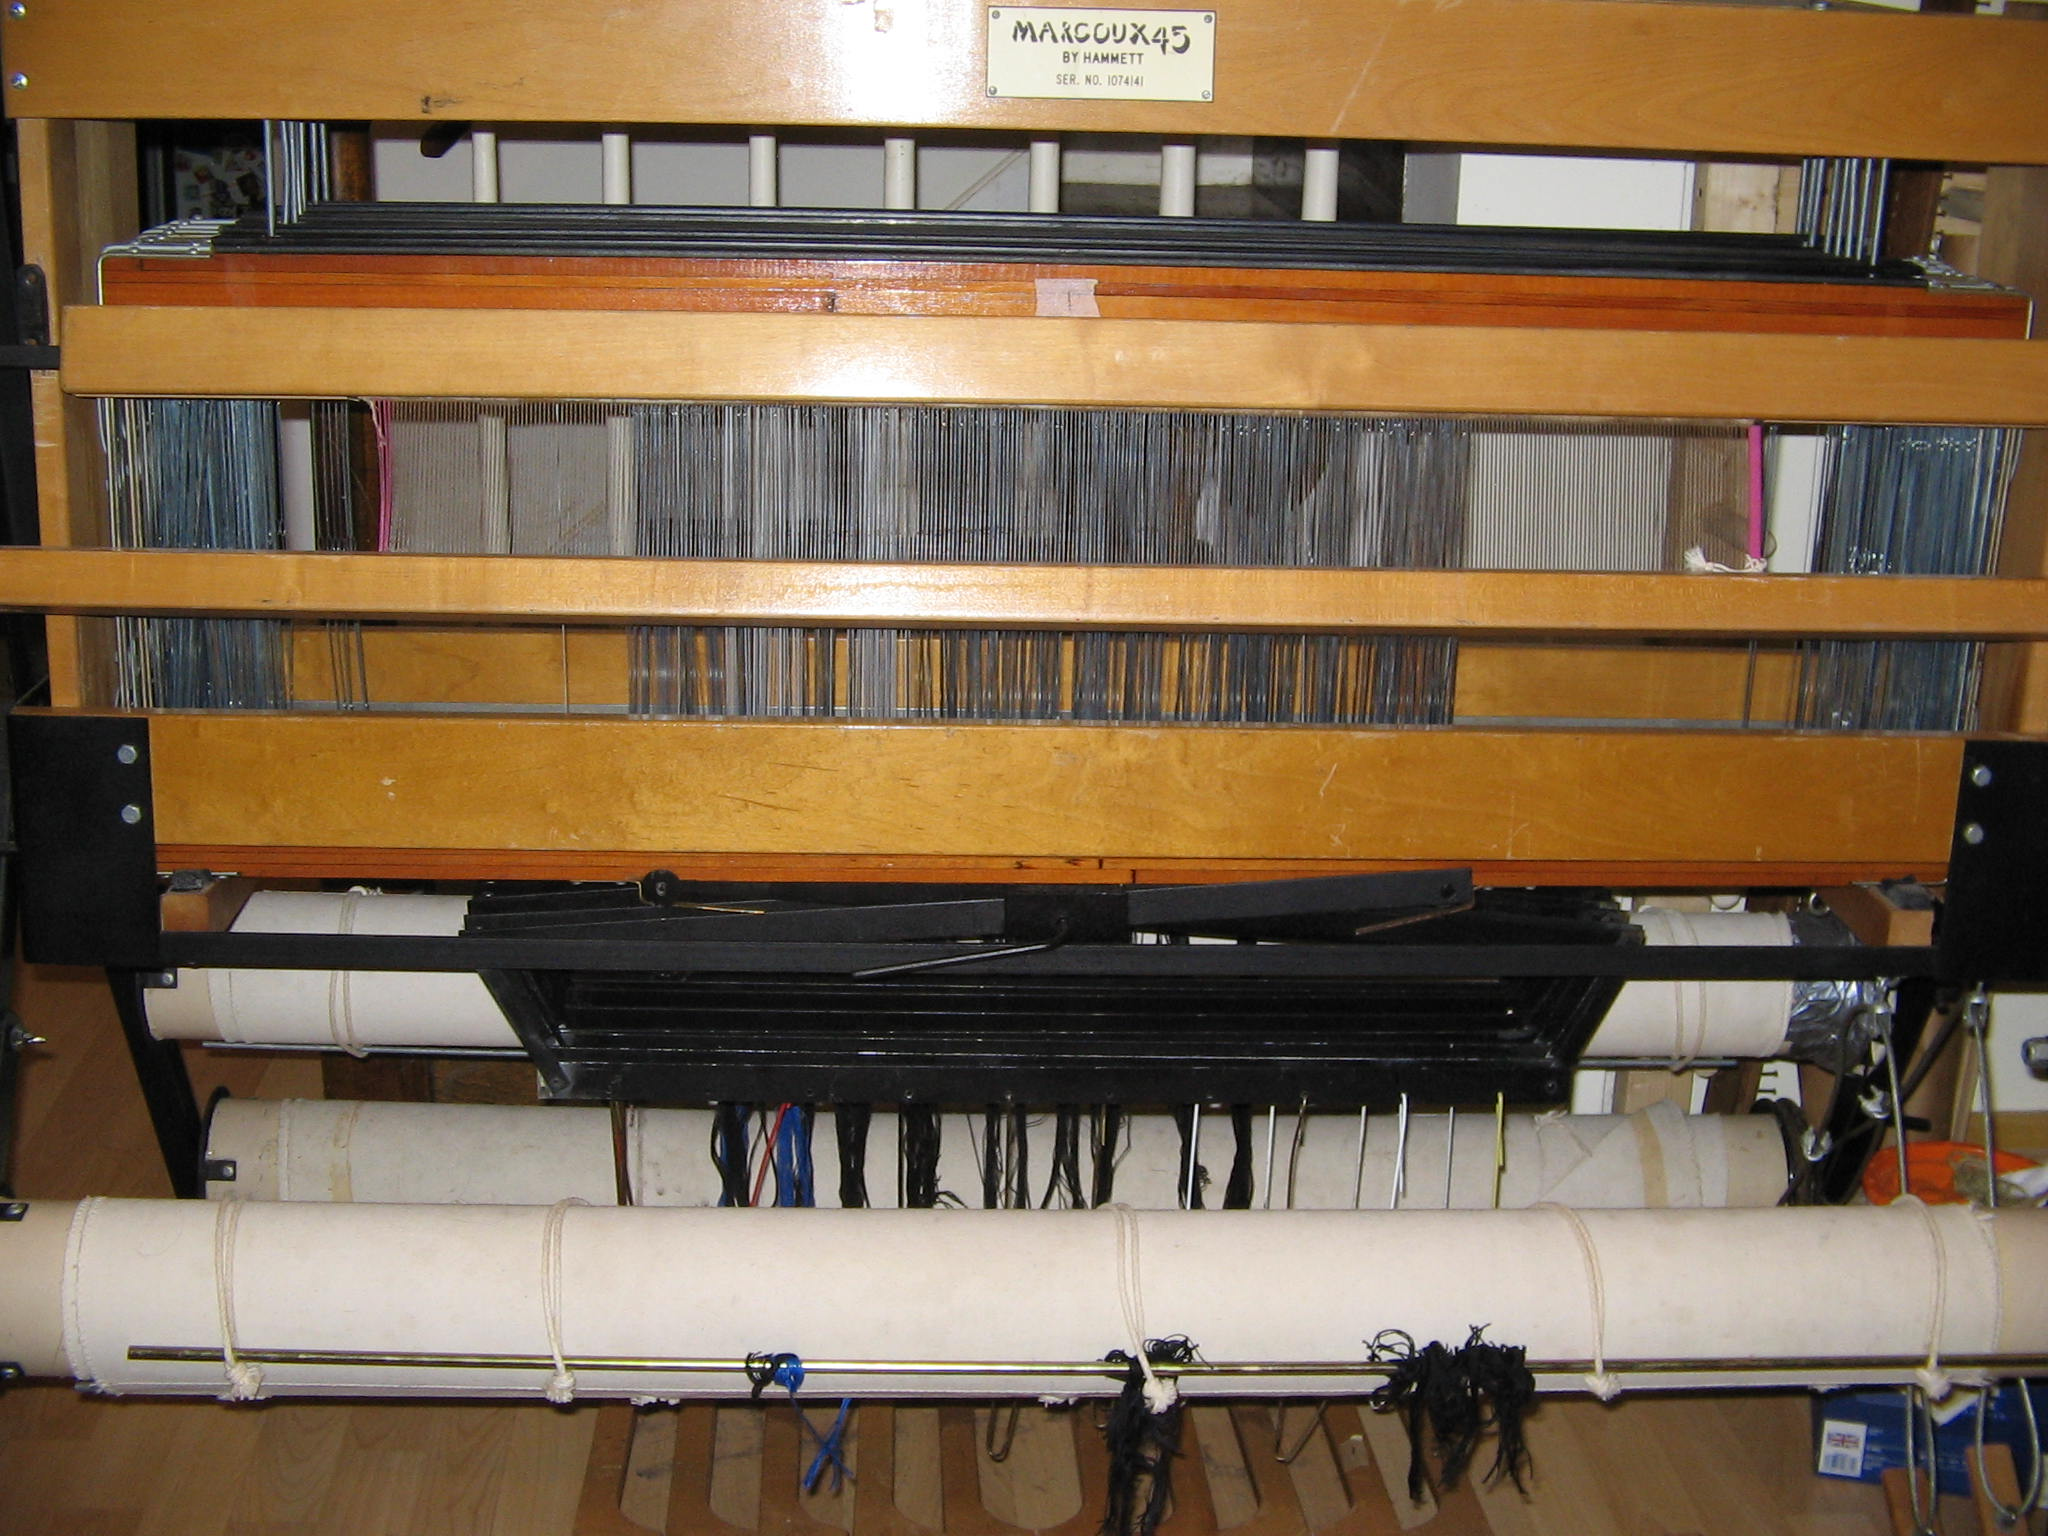
\includegraphics[width=0.8\linewidth]{images/loom.png}
\caption{A loom
                \label{fig-loom}}
\end{figure}
Weaving that is considered here is what can be realized with a multi-harness loom such as the one shown in \hyperref[fig-loom]{Figure~\ref{fig-loom}}.
The main topics are %
\leavevmode%
\begin{itemize}[label=\textbullet]
\item{}an exposition of how the weaver's draft, consisting of a tie-up draft, treadlig matrix and lift plan can
		 be combined to visualize the final weave that will be produced, and%
\item{}an analysis of how harnesses can be tied in such a way to realize a given weave pattern.%
\end{itemize}
\typeout{************************************************}
\typeout{Subsection 1.1 Weaving Basics}
\typeout{************************************************}
\subsection[Weaving Basics]{Weaving Basics}\label{ss-weaving-def}
\index{Weaving Basics}A weave pattern is created by interleaving two sets of parallel lengths of fiber. Each of the fibers in one set, the \terminology{warp}, is connected to exactly one of \(n\) harnesses, \(n \geq 2\). Each \terminology{harness} will lift the threads that are connected to it.  A series of \terminology{treadles} are connected to the harnesses, with each treadle connected to between 1 and \(n-1\) of the harnesses. When a treadle is pressed, the warp fibers connected to that treadle through the harnesses are lifted, forming a \terminology{shed} between the warp fibers that are lifted and those that are not lifted. A \terminology{weft} thread can then be passed through the shed.  The weft runs perpendicular to the warp. Normally, the weft thread is passed through the shed with a \terminology{shuttle}. %
\par
By performing a sequence of pedal presses and shuttle passes that interleave the warp with the weft, a weaving pattern is realized.  Using different colors for the warp and weft makes the pattern visible. In this discussion we only consider "monochromatic weaving," where the warp are all of one color and the weft threads are all of a second color.%
\typeout{************************************************}
\typeout{Subsection 1.2 The Weaver's Draft}
\typeout{************************************************}
\subsection[The Weaver's Draft]{The Weaver's Draft}\label{ss-weaving-draft}
A weaver's draft is typically a array of four matrices, such as the small example in \hyperref[fig-draft]{Figure~\ref{fig-draft}}. The top left (A) matrix, called the harness draft, has as many columns as the number of warp threads, and there is a row for each harness.  Each column indicates to which harness the corresponding thread is tied. Each thread is tied to only one harness and so each column has one mark.  The top right (B) matrix, called the pedal plan, indicates which harnesses are tied to each treadle and determines which threads will make up the top of the shed when a pedal is pressed. The pedal has as many rows as there are harnesses and as many columns as there are pedals.  The bottom right (C) matrix is the lift plan, which indicates the sequence of pedal presses that are to performed for each successive weft thread. The lift plan has as many columns as there are pedals.  The number of rows is the number of weft threads, although the lift plan is frequently periodic and the rows on the draft would be repeated. The output from is sequence of presses and shuttle movements is indicated with the bottom left (D) matrix, the weave.  Some weavers use different  positioning schemes in their drafts, but the essential information is the same.  %
\leavevmode%
\begin{figure}
\centering
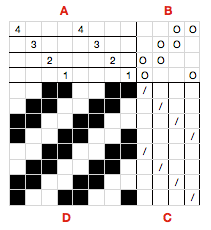
\includegraphics[width=0.8\linewidth]{images/fig-draft.png}
\caption{A typical monochromatic weaving draft
                \label{fig-draft}}
\end{figure}
\typeout{************************************************}
\typeout{Subsection 1.3 Computing the weave pattern}
\typeout{************************************************}
\subsection[Computing the weave pattern]{Computing the weave pattern}\label{subsection-3}
Clearly the weaver has control over the harness matrix, pedal matrix and lift plan.   It is a simple matter of logic to determine whether any weft thread will lie above or below any warp thread.  In \hyperref[section-products]{Section~\ref{section-products}} we derive formulas to determine the whole weave based on matrix multiplication.%
\par
Not every draft will produce a weave that "hangs together."  A trivial example would be a draft for which one of the warp fibers is always on the upper part of the shed, which would leave that thread to float around.  Less obvious cases can arise though.  We will describe how this can be determined from the output matrix.%
\typeout{************************************************}
\typeout{Subsection 1.4 Realization of a Weave}
\typeout{************************************************}
\subsection[Realization of a Weave]{Realization of a Weave}\label{subsection-4}
An even more practical question is how to specify the harness matrix, pedal matrix and lift plan to attain a specific weave pattern, if at all possible for a given loom.  In \hyperref[section-realization]{Section~\ref{section-realization}}, we give a description of how to determine whether one can  realize a desired weave pattern and how the loom can be set to do so.%
\typeout{************************************************}
\typeout{Section 2 Weaving as a product of matrices}
\typeout{************************************************}
\section[Weaving as a product of matrices]{Weaving as a product of matrices}\label{section-products}
Recall that a weaving draft is a block array with the stucture


\(\begin{array}{|c|c|}
\hline
 H &P \\
\hline
 W &L \\
\hline
\end{array}\)

where \(H, T, W \textrm{ and } L\) are boolean matrices defined as follows, where True is represented as 1 and False as 0.  Expressions that derive the main formula in this section use the notation of Boolean arithmetic, were conjunction (``and'') is denoted by \(\cdot\) and disjunction (non-exclusive ``or'') is denoted by \(+\).%
\par
 \(H\)  is the harness draft it has as many rows as a loom has harnesses and as many columns as the number of warp threads. We define entries of this matrix by
\begin{equation*}H_{i j }=\textrm{ Is harness } i \textrm{ connected to  warp thread } j?\end{equation*}
%
\par
\(P\)  is the pedal matrix it has as many rows as a loom has harnesses and as many columns as the number of treadles in the loom. We define entries of this matrix by
\begin{equation*}P_{i j}= \textrm{Is harness } i \textrm{ lifted by treadle } j?\end{equation*}
%
\par
 \(L\)  is the lift plan matrix it has as many rows as the number of threads in the weft and as many columns as the number of treadles in the loom. We define entries of this matrix by
\begin{equation*}L_{i j}= \textrm{Is treadle } j \textrm{ pressed for weft tread } i?\end{equation*}
%
\par
 \(W\) is the matrix of the weave resulting  from the setting of  \(H\) ,  \(P\) , and  \(L\) . We derive  \(W\)  as a matrix
product in terms of these settings.
\begin{equation*}W_{i j}= \textrm{Is warp thead } j \textrm{ lifted above weft thread } i?\end{equation*}%
\begin{claim}[The main formula]\label{claim-1}
 \(W = L T^t H\) , where \(T^t\) is the transpose of \(T\).%
\end{claim}
\begin{proof}\hypertarget{proof-1}{}
To prove our claim we define the matrix  \(C\),  where \begin{equation*}C_{i j}= \textrm{Is warp thead } j \textrm{ lifted when treadle } i \textrm{ is pressed?}\end{equation*}%
\par
We derive a formula for the \(C\):
\begin{equation*}
\begin{split}
C_{i j} &= \textrm{Is warp thead } j \textrm{ lifted when treadle } i \textrm{ is pressed?}\\
	  	& = P_{1i}H_{1j }+P_{2i}H_{2j }+\cdots \\
		& = H^t{}_{j 1}P_{1 i}+H^t{}_{j 2}P_{2 i} +\cdots \\
		& = \left( H^t P \right)_{j i}\\
		& = \left( H^t P \right)^t_{i j}\\
		& = \left(T^tH\right)_{i j}
\end{split}
\end{equation*}
%
\par
Now we can compute \(W\).
\begin{equation*}
\begin{split}
W_{i j} &= \textrm{Is warp thead } j \textrm{ lifted above weft thread } i?\\
		&= L_{i 1}C_{1j }+ L_{i 2}C_{2j }+\cdots \\
		& = (L C)_{i j}\\
		&= \left(L T^tH\right){}_{i j}
\end{split}
\end{equation*}
%
\end{proof}
\typeout{************************************************}
\typeout{Section 3 Realization of a Weave Pattern}
\typeout{************************************************}
\section[Realization of a Weave Pattern]{Realization of a Weave Pattern}\label{section-realization}
\index{Minsets} 
Whether a pattern can be realized is determined by whether each of the distinct horizontal rows of the pattern can be realized. Let \(r_1,\dots , r_n\) be those rows. Each row \(r_i\) is realized be lifting a set \(R_i\) of warp fibers. Give two warp fibers \(f_1\) and \(f_2\), if \(f_1, f_2 \in R_i\) for some \(i\) yet \(f_1 \in R_j\) while \(f_2 \notin R_j\), we cannot connect \(f_1\) and \(f_2\) to the same harness.   If we presume that all warp fibers are connected to exactly one harness, with the set of warp fibers connected to harness \(i\) equal to \(H_i\), then the warp fibers lifted to realize a row must be a union of the \(H_i's\). These observations imply that \(\{H_i\}\) would be the minsets generated by \(\{R_j\}\).  For each \(i\),

\begin{equation*}H_i = \bigcap_{j=1}^{n}{\tilde{R}_j}\end{equation*} 
where \(\tilde{R}_j\) is either \(R_j\)  or \(R_j^c\).
%
%
\appendix
%
\typeout{************************************************}
\typeout{Appendix A Notation}
\typeout{************************************************}
\section[Notation]{Notation}\label{appendix-1}
This is some notation introduced in the article.%
\begin{longtable}[l]{llr}
\textbf{Symbol}&\textbf{Description}&\textbf{Page}\\[1em]
\endfirsthead
\textbf{Symbol}&\textbf{Description}&\textbf{Page}\\[1em]
\endhead
\multicolumn{3}{r}{(Continued on next page)}\\
\endfoot
\endlastfoot
\end{longtable}
\typeout{************************************************}
\typeout{References  References}
\typeout{************************************************}
\section*{References}\label{references-1}
\addcontentsline{toc}{section}{References}
%% If this is a top-level references
%%   you can replace with "thebibliography" environment
\begin{referencelist}
\bibitem[1]{biblio-rasmussen-harness}\hypertarget{biblio-rasmussen-harness}{}Shelley Rasmussen, \textit{On 3-Harness Weaving: Cataloging Designs Generated by Fundamental Blocks Having Distinct Rows and Columns}.The Electronic Journal of Combinatorics, 2008, \textbf{15} no.\@\,R1, 57\textendash{}62.
                
\end{referencelist}
%
%% The index is here, setup is all in preamble
\printindex
%
This article was authored in MathBook XML.%
\end{document}